\subsection{Frontend Arkitektur}

Frontend applikationen vil have til formål at håndtere brugerinput og output. Dvs. at der i Frontenden vises det data fra gamelogic, som brugeren skal have, og at det præsenteres på en overskuelig og brugervenlig måde. Dette resulterer i at brugeren kan forstå og kan finde ud af at bruge spillet på den tiltænkte måde.
Derudover skal Frontenden tage hånd om bruger input, og sørge for at brugeren giver korrekt input og at der tages hånd om eventuelt forkert input.\\
Da der er mange forskellige menuer og skærme i spil i frontenden er der lavet følgende C3 model for Frontenden (\autoref{fig:Arkitektur-FrontEnd-C3}), som giver en idé om hvilke skærme og menuer der kan gå til hvilke andre menuer/skærme. Udover dette fortæller modellen også om hvordan og hvilke skærme og menuer der snakker med noget uden for frontenden selv f.eks. skal der ved Login/Register kontaktes databasen for at få verificeret logind-oplysninger, og samtidig skal der ved save og load-game hentes en liste af gemte spil i databasen hvorefter der skal henholdsvis skrives og hentes fra databasen alt efter om man gemmer eller henter et spil. Der skal hertil nævnes at Login og Register står til at snakke med backenden direkte og ikke igennem gamelogic blokken, dette er valgt da funktionen ikke kaldes i gamelogic blokken, men den kaldes direkte i backend controlleren. Derudover er modellen mere overskuelig på denne måde og fungerer bedre til at give overblik over navigationen igennem menuerne.

\begin{figure}[H]
\centering
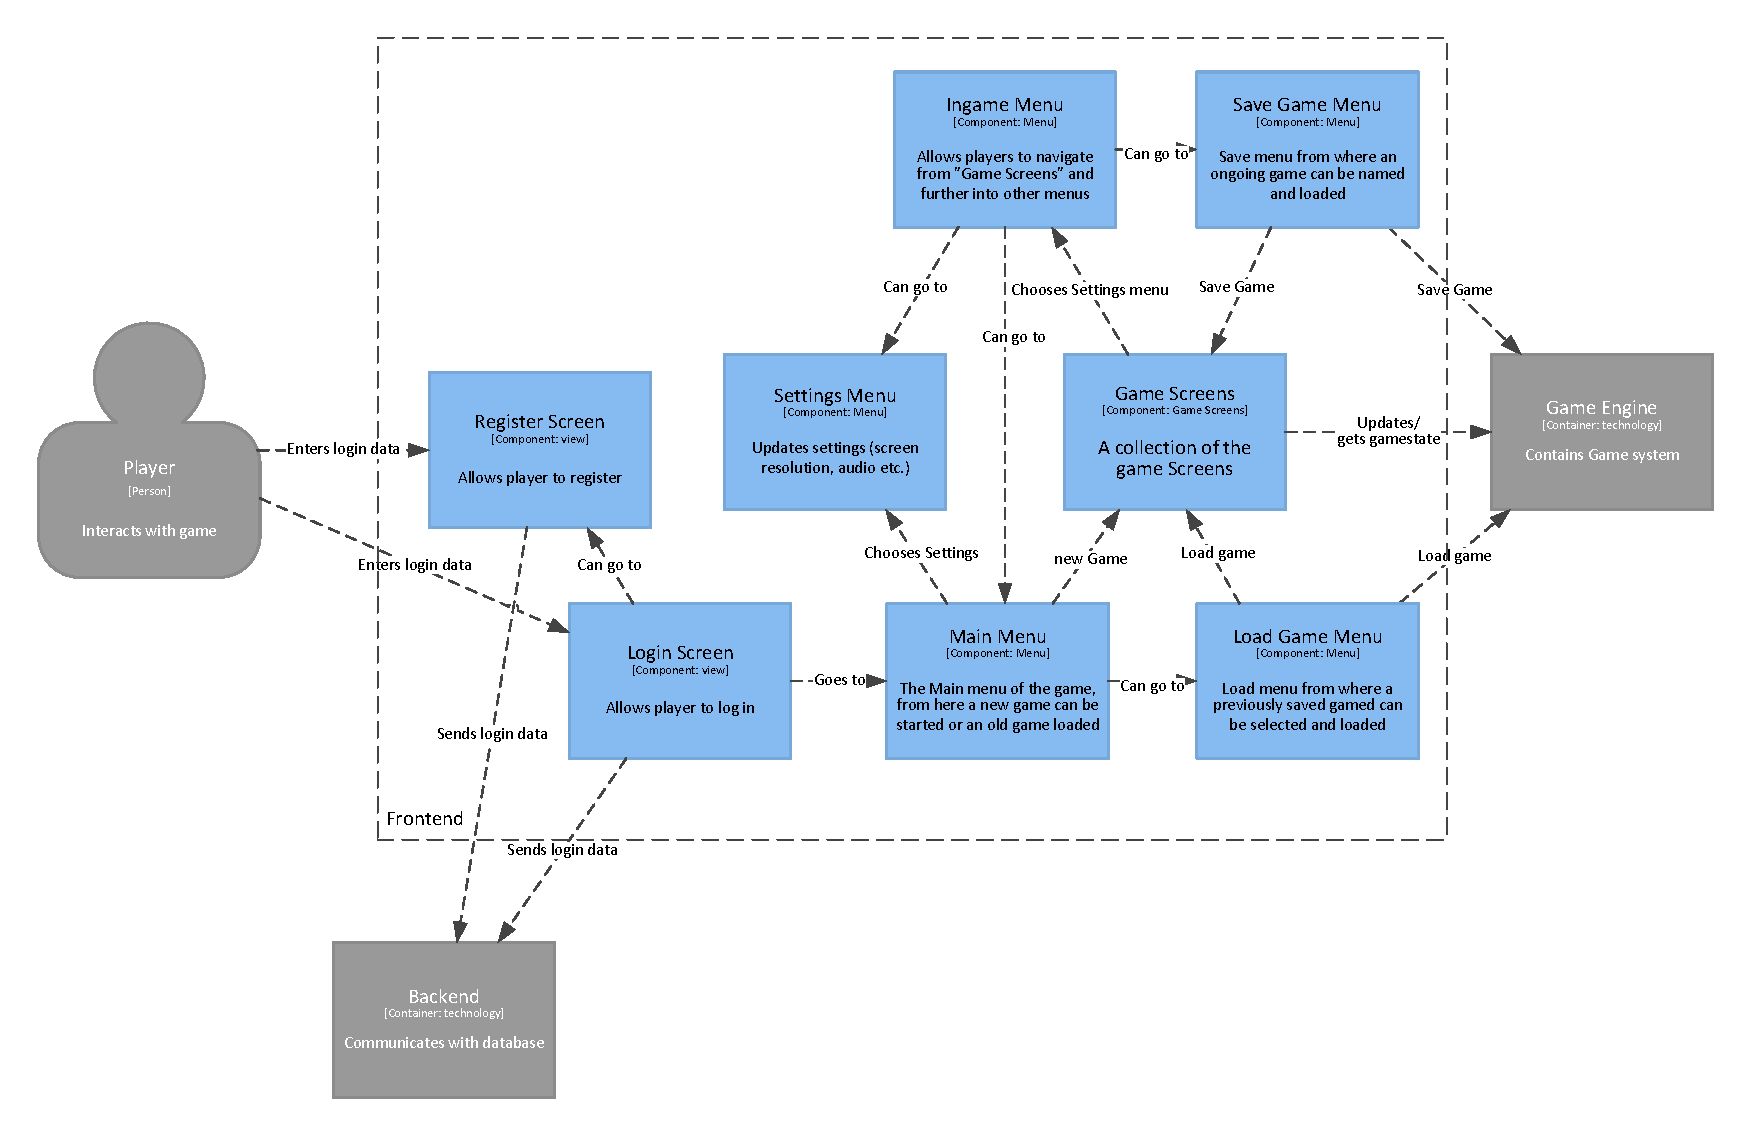
\includegraphics[width = \textwidth]{02-Body/Images/Frontend_C3.pdf}
\caption{C3-Model for Frontend. Modellen fortæller hvordan man kan navigere igennem forskellige menuer og hvilke menuer der kan føre til hvad. Derudover kan man se hvilke blokke der snakker ud af frontenden og sammen med resten af systemet.}
\label{fig:Arkitektur-FrontEnd-C3}
\end{figure}

\subsubsection{Pseudo Frontend Arkitektur}
(Hovedrapport stuff)
For at give overblik over, hvordan kommunikationen mellem frontend, backend og gamecontroller kommer til at foregå, er der lavet et pseudo sekvensdiagram for følgende UserStories:
\\
- Login\\
- Register\\
- Save Game\\
- Load Game\\
(/Hovedrapport stuff)
Der er ikke lavet sekvensdiagrammer for alle af projektets userstories, da mange af disse fungerer på samme måde og derfor ikke bidrager med noget nyt ift. dokumentationen.
Nedenfor ses pseudo sekvensdiagrammer for de fire userstories:\\
- Login\\
- Register\\
- Save Game\\
- Load Game\\

\noindent Først ses "Login"(\autoref{fig:Arkitektur-FrontEnd-Login}), som viser forløbet af userstory "Login", med en reference til userstory "Register", hvis brugeren ikke er registreret i forvejen. Udover dette er der ydermere vist håndtering fejlet login. Det skal her nævnes at brugeren kan ikke spille spillet uden at logge ind først, der tillades ikke at spillet kan spilles i Offline-tilstand.\\

\begin{figure}[H]
\centering
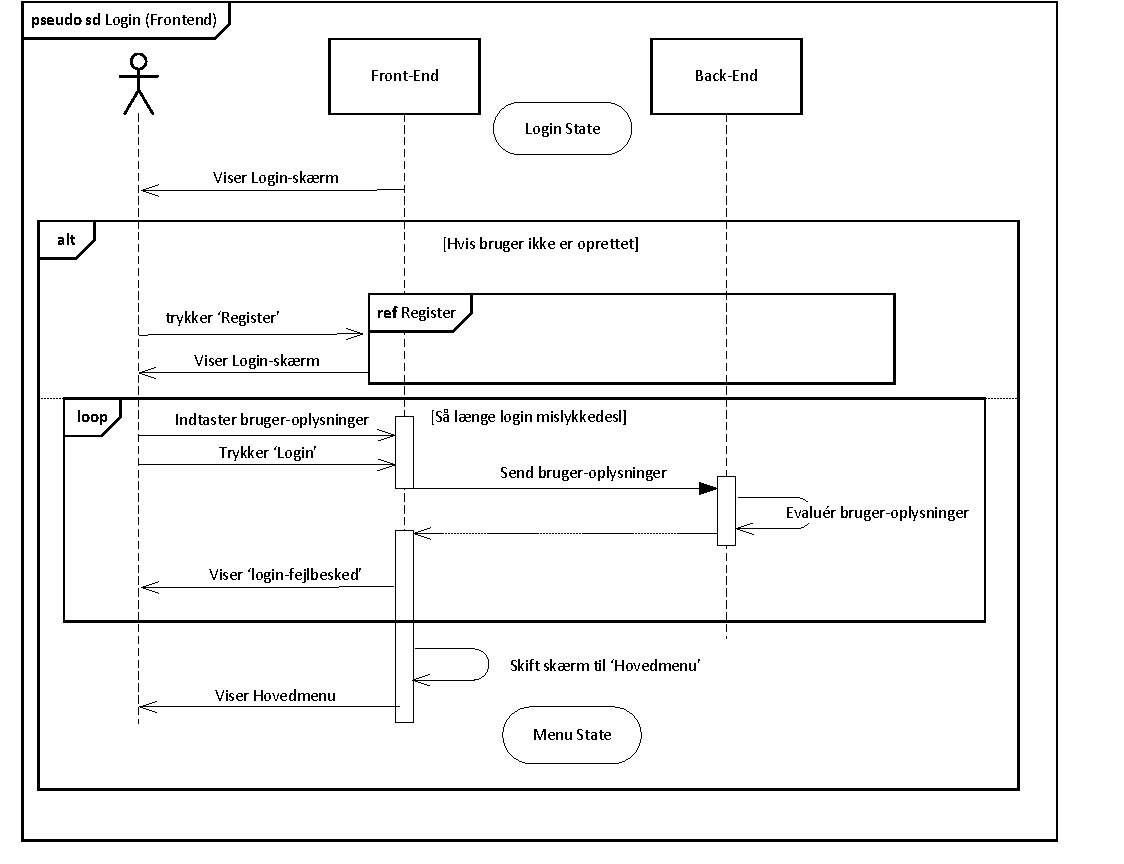
\includegraphics[width = \textwidth]{02-Body/Images/Front-End_-_Arkitektur-login.pdf}
\caption{Pseudo sekvensdiagram af forløbet af userstory "Login", set fra Frontends perspektiv. Med reference til "Register" userstory og håndtering af forkerte login oplysninger.}
\label{fig:Arkitektur-FrontEnd-Login}
\end{figure}

\noindent Dernæst ses "Register" (\autoref{fig:Arkitektur-FrontEnd-Register}), som viser forløbet af hvordan en bruger kan registrere sig med en profil i systememt. Der kan ses på \autoref{fig:Arkitektur-FrontEnd-Login}, at hvis en bruger ikke er oprettet skal man gøre dette først. Derefter skal man vælge et brugernavn og kodeord, hvis brugernavnet er ledigt og alt ellers går godt, kommer man tilbage til "Login" skærmen. ellers får man en fejlbesked på skærmen og bliver bedt om at prøve med et andet brugernavn.\\

\begin{figure}[H]
\centering
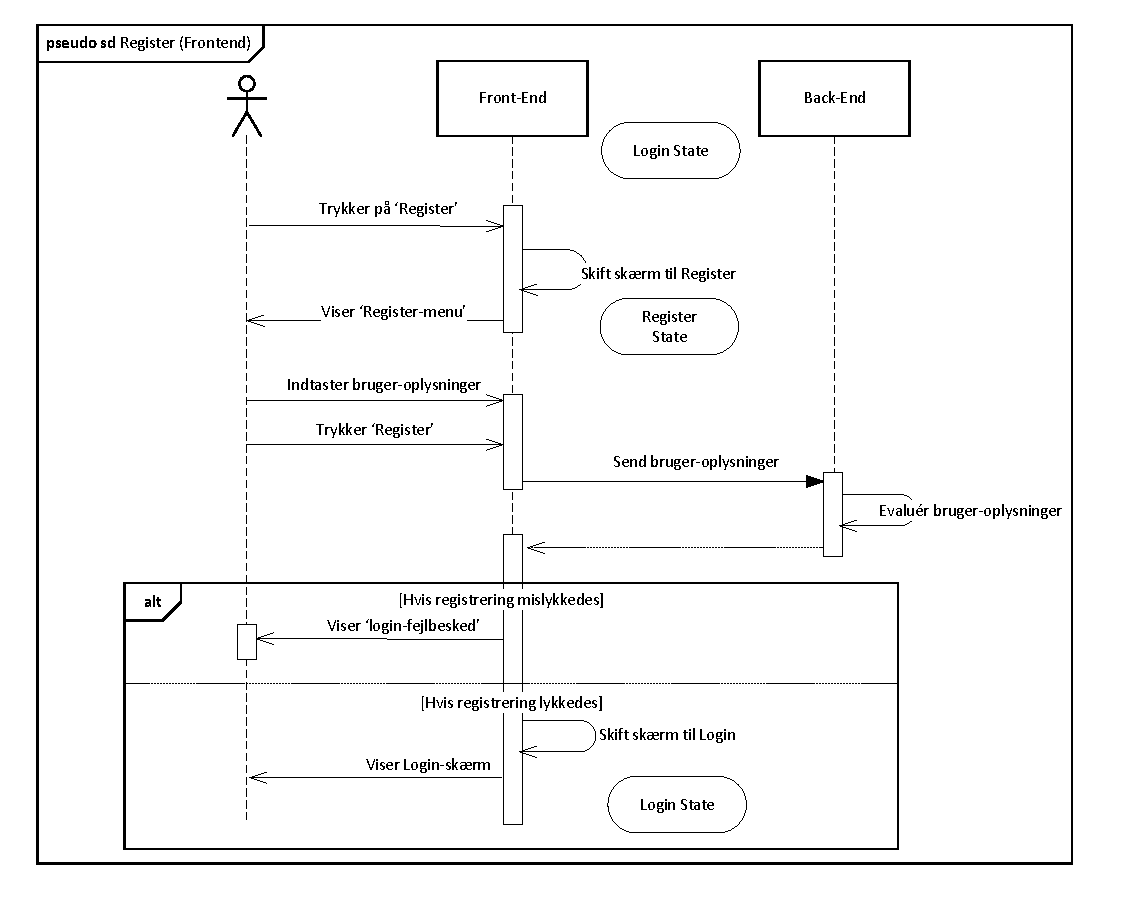
\includegraphics[width = \textwidth]{02-Body/Images/Front-End_-_Arkitektur-register.pdf}
\caption{Pseudo sekvensdiagram af forløbet af userstory "Register", set fra Frontends perspektiv. Med håndtering af forkerte login oplysninger.}
\label{fig:Arkitektur-FrontEnd-Register}
\end{figure}

\noindent På \autoref{fig:Arkitektur-FrontEnd-Save} ses "Save Game", som viser forløbet når en bruger gerne vil gemme sit igangværende spil, set fra Frontends perspektiv. Her kan man bide mærke i, at når der skiftes skærm, vil den nye skærm få initialiseret sine variabler i sin constructor og derfor er der kun et selv kald hver gang skærmen skiftes.
Hertil skal der nævnes at hvis brugeren er i "Combat State" er det ikke muligt at gemme spillet og knappen "Save Game" på "In Game Menu" vil ikke kunne ses eller bruges.\\

\begin{figure}[H]
\centering
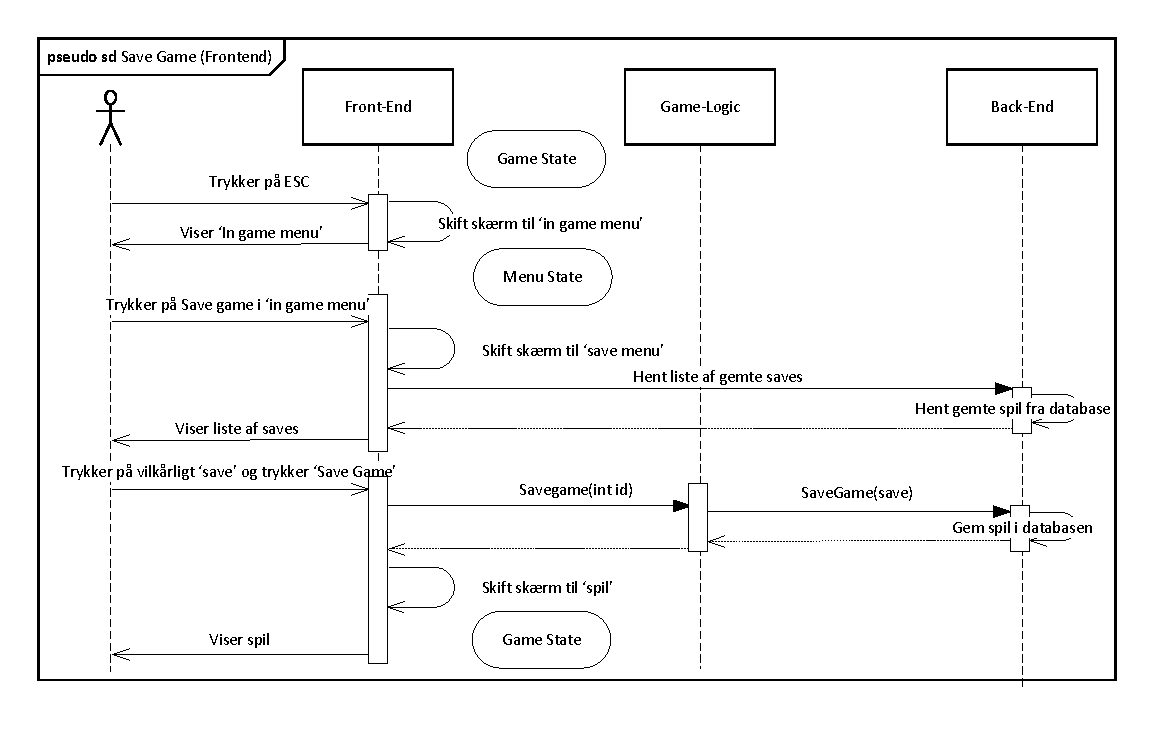
\includegraphics[width = \textwidth]{02-Body/Images/Front-End_-_Arkitektur-savegame.pdf}
\caption{Pseudo sekvensdiagram af forløbet af userstory "Save Game", set fra Frontends perspektiv. Der laves 2 kald til databasen igennem Backenden, hvori der i det første kald,  "Hent liste af gemte saves" hentes en liste af brugerens gemte spil og i andet kald gemmes brugerens nuværende spil henover det valgte spil.}
\label{fig:Arkitektur-FrontEnd-Save}
\end{figure}

\noindent Tilsidst kan der på \autoref{fig:Arkitektur-FrontEnd-Load} ses "Load Game", som viser forløbet når en bruger gerne vil hente et tidligere gemt spil fra databasen, set fra Frontends perspektiv. Denne userstory minder på mange måder om "Save Game", men i stedet for at sende et element til databasen, skal der hentes et gemt spil fra databasen, med alle de data der skal bruges for at kunne loade sit spil op præcis som man forlod det. \\

\begin{figure}[H]
\centering
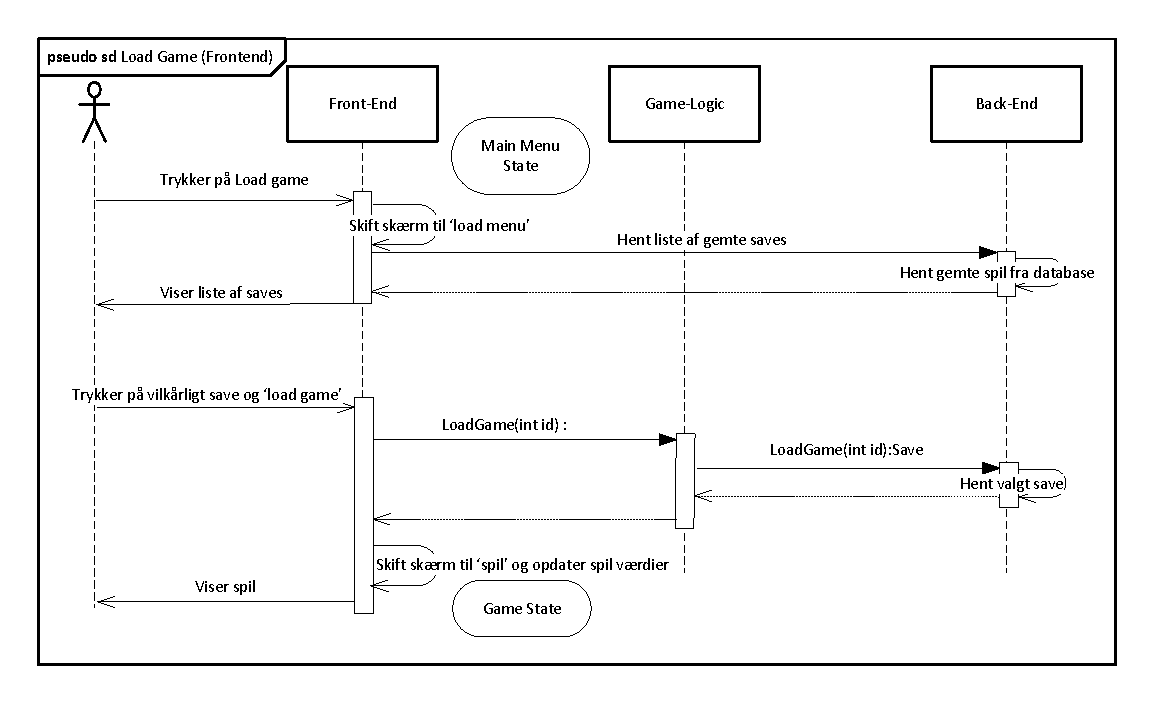
\includegraphics[width = \textwidth]{02-Body/Images/Front-End_-_Arkitektur-loadgame.pdf}
\caption{Pseudo sekvensdiagram af forløbet af userstory "Load Game", set fra Frontends perspektiv. Der laves 2 kald til databasen igennem Backenden, hvori der i det første kald,  "Hent liste af gemte saves" hentes en liste af brugerens gemte spil og i andet kald hentes  brugerens valgte spil og spillet startes op.}
\label{fig:Arkitektur-FrontEnd-Load}
\end{figure}

\newpage
